\documentclass[../report.tex]{subfiles}
\begin{document}
\graphicspath{{img/}{../img/}}

\section{Overview}
This chapter will describe important implementation details of Ocon. The system is realized by three main components. A central, a widget and a client. In addition a communication library have been created to facilitate distributed communication between the three components.


\section{Encapsulation of Context}

Entities are generalized by the interface IEntity, specifying general information for all entities. AbstractEntity extends on IEntity and overrides ToString() with a meaningful implementation. Both are public and it is up the an implementer which to extend.

On figure \ref{fig:PersonImplementation} is an example of Person extending AbstractEntity with a present property motivated by the need for this context information.


\begin{figure}[H]
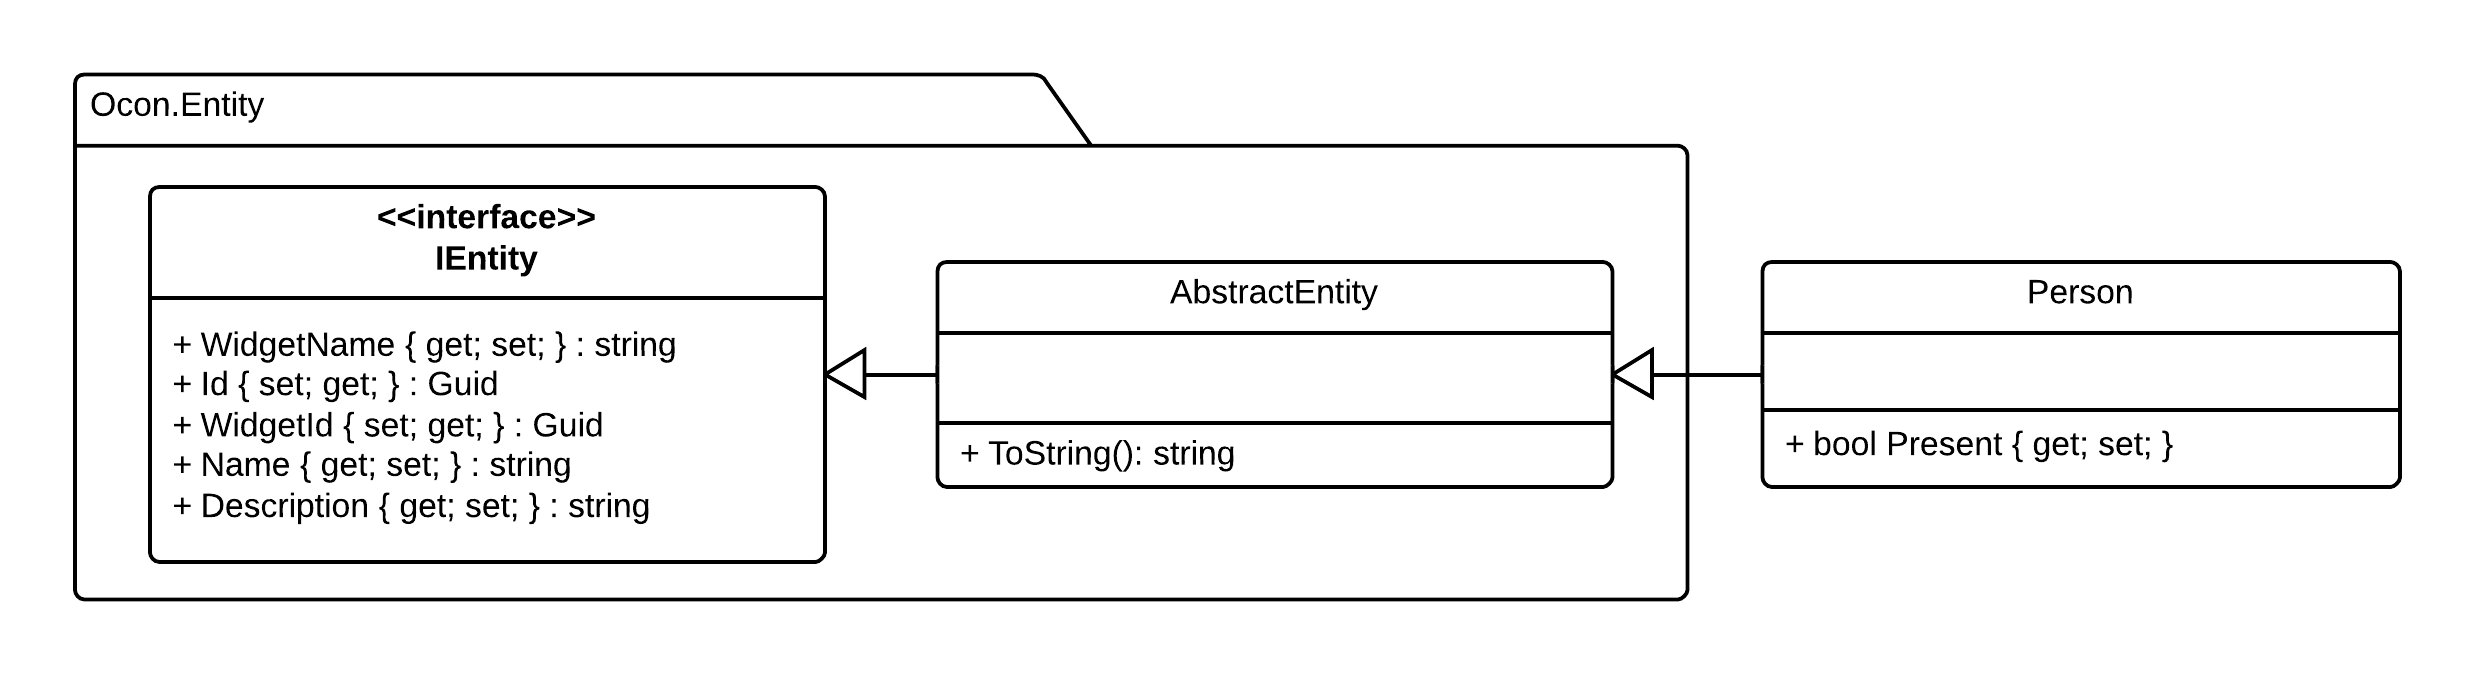
\includegraphics[width=\linewidth]{customEntityClass.png}
\caption{Person as a custom IEntity implementation}
\label{fig:PersonImplementation}
\end{figure}


\section{Communication}

To support the design decision that the communication part should be injectable the communication have been interfaced in IOconCom. (The interface can be seen in figure \ref{fig:oconclassdiagram})

Ocon contains a default communication implementation build using the TCP/IP layer. For serialization we have chosen to use JSON. These decisions have been made so that developers are not bound to the .NET platform and can make clients and widgets in other languages like Java, or C directly on a micro controllers like Arduino.

For peer discovery we have chosen to use IP multicast. The central broadcasts itself for peers to discover. The peer, clients and widgets, is listening on the multicast endpoint and will invoke an event when a central is discovered.

To facilitate discovery OconTcpCom implements two methods: Broadcasting and DiscoveryService. Both methods are running on threads. This is done so that that peers are not blocked when broadcasting or discovering. When a peer is discovered an DiscoveryService event will be fired to notify subscribers.

To listen and send for sending Entites, situation updates and situation subscription following methods have been implemented: Listen, SendEntity, SendSituationState, and SubscribeSituaion. When listen is called a new thread is started and whenever a message is received either IncommingSituationSubscribtionEvent, IncommingEntityEvent, or IncommingSituationChangedEvent is fired to notify subscribers. Then different send methods are also executed on a thread. This have been done to avoid blocking and to get faster execution time as multiple messages can be sent at the same time.

The send methods take a peer. The peer is a helper class. Just like entities, peers are assigned a GUID. The GUID is a unique identifier for the peer and the communication class stores the IPEndPoints associated with the GUIDs. When a message from a peer is received or discovered the IpEndPoint is saved in a HashSet. By doing this messages can be sent only by using the peer and not the IPEndPoint which adds an abstraction layer to the module. 

\section{OconWidget}
\label{sec:OconWidget}

The OconWidget's purpose is to track entities and keep them updated in the central. The widget developer should translate sensor input to entities and then the Ocon widget will facilitate tracking the entity and sending it to the central. (See figure \ref{fig:widgetComHelper})

\begin{figure}
\hspace{-70px}
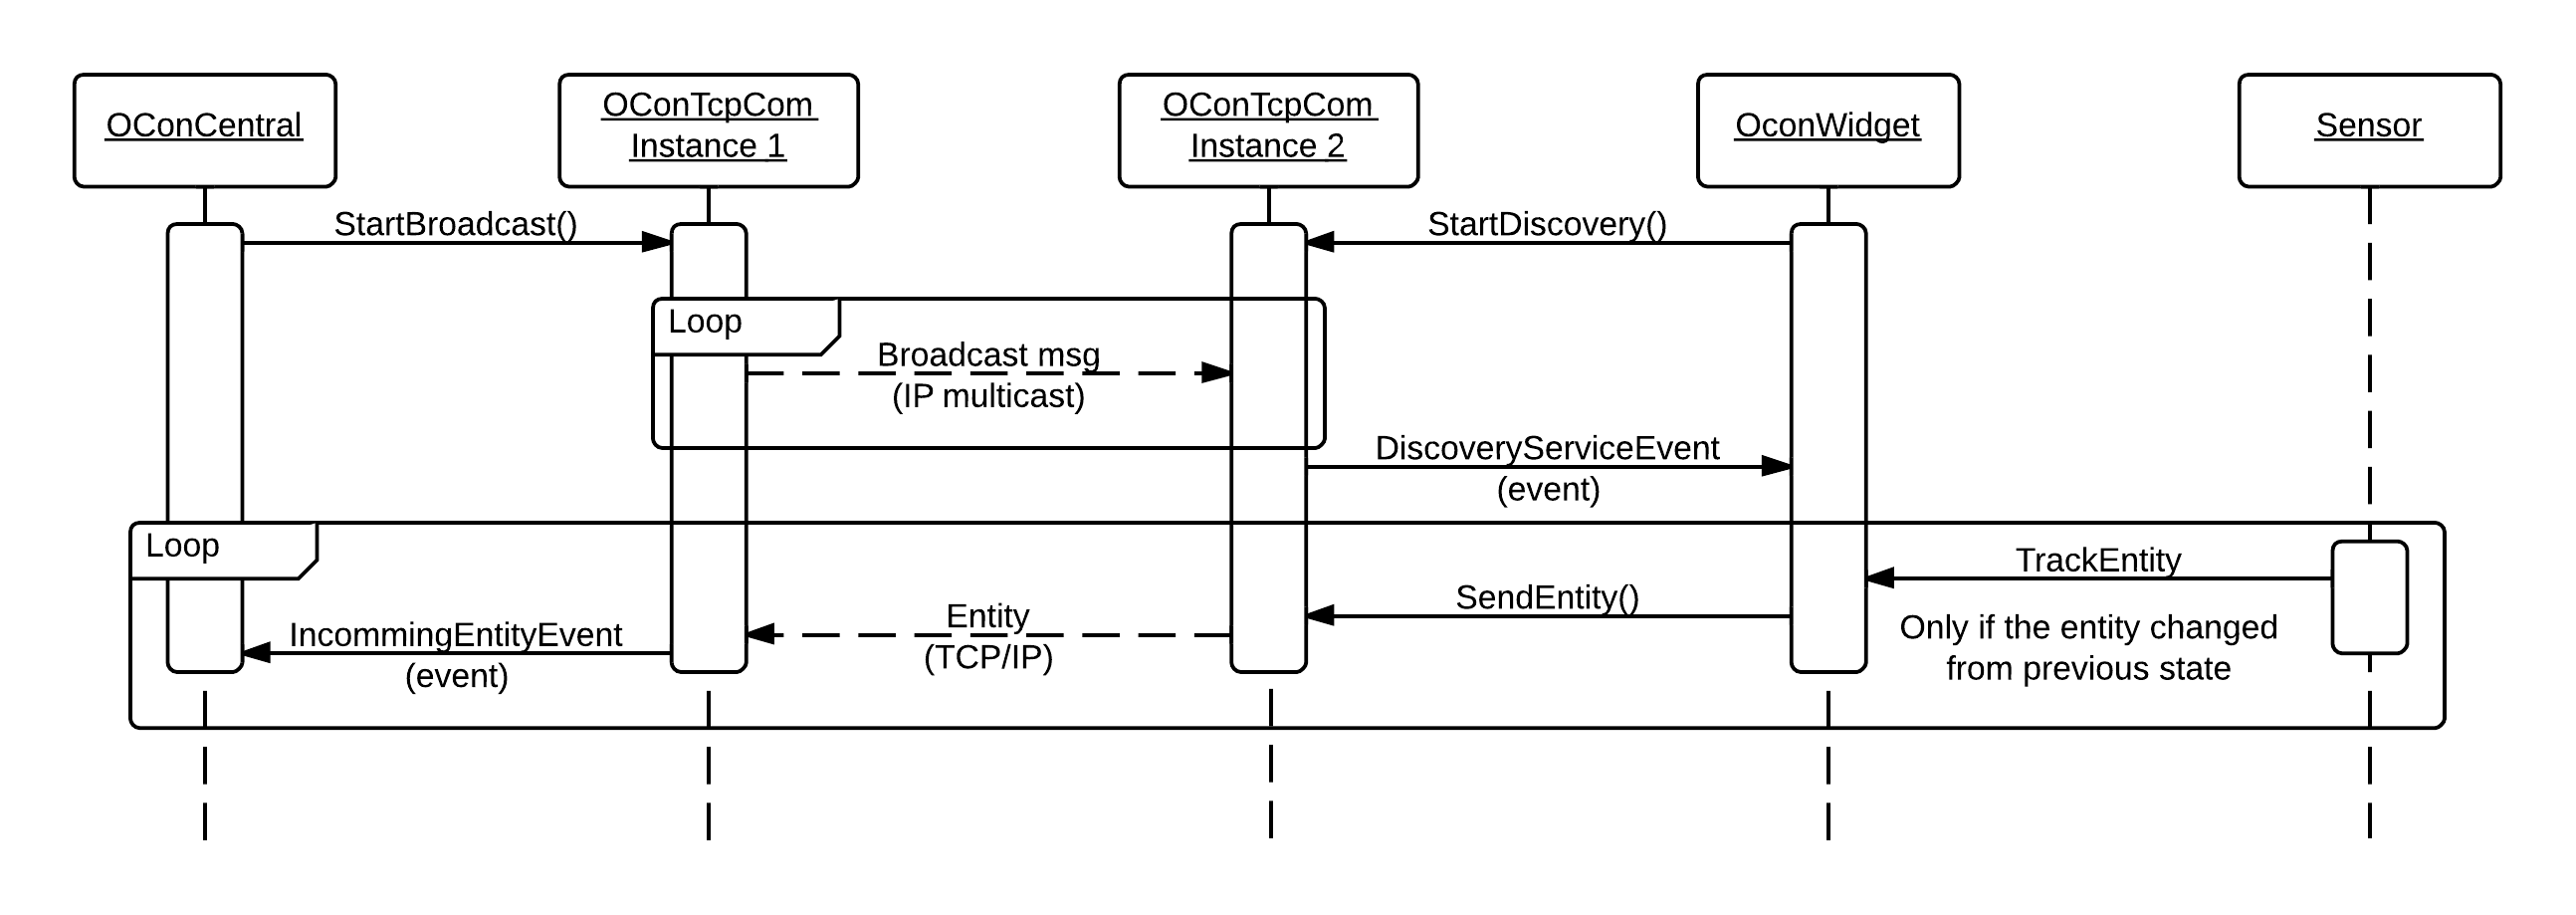
\includegraphics[width=500px]{comHelperSequence-widget.png}
\caption{Widget to Central sequence diagram}
\label{fig:widgetComHelper}
\end{figure}

The OconWidget is very light. When constructed the widget will listen for OconCentrals by starting discovery and subscribing to DiscoveryServiceEvents on the IOconCom. When a central is found an event will be fired and the central will be added as subscriber. OconWidget has only one methods. Notify(IEntity entity). When Notify is called from the sensor a check weather or not the entity is already tracked is performed. If not tracked it will be allocated a new GUID before it is sent to the central through the communication module. The GUID is a unique ID used for distributed systems and allows Ocon to distinguish between adding the entity as a new entity or updating an entity already know to the framework. The usage of the widget is very easy for application developers as they only have to use one method when sending new entities to the central.

\section{OconClient}
The OconClient's purpose is to sent predicates to the central for tracking. When a situation update is send from the central the client must be able to notify the parent application about the situation update. (See figure \ref{fig:clientComHelper})

\begin{figure}
\hspace{-70px}
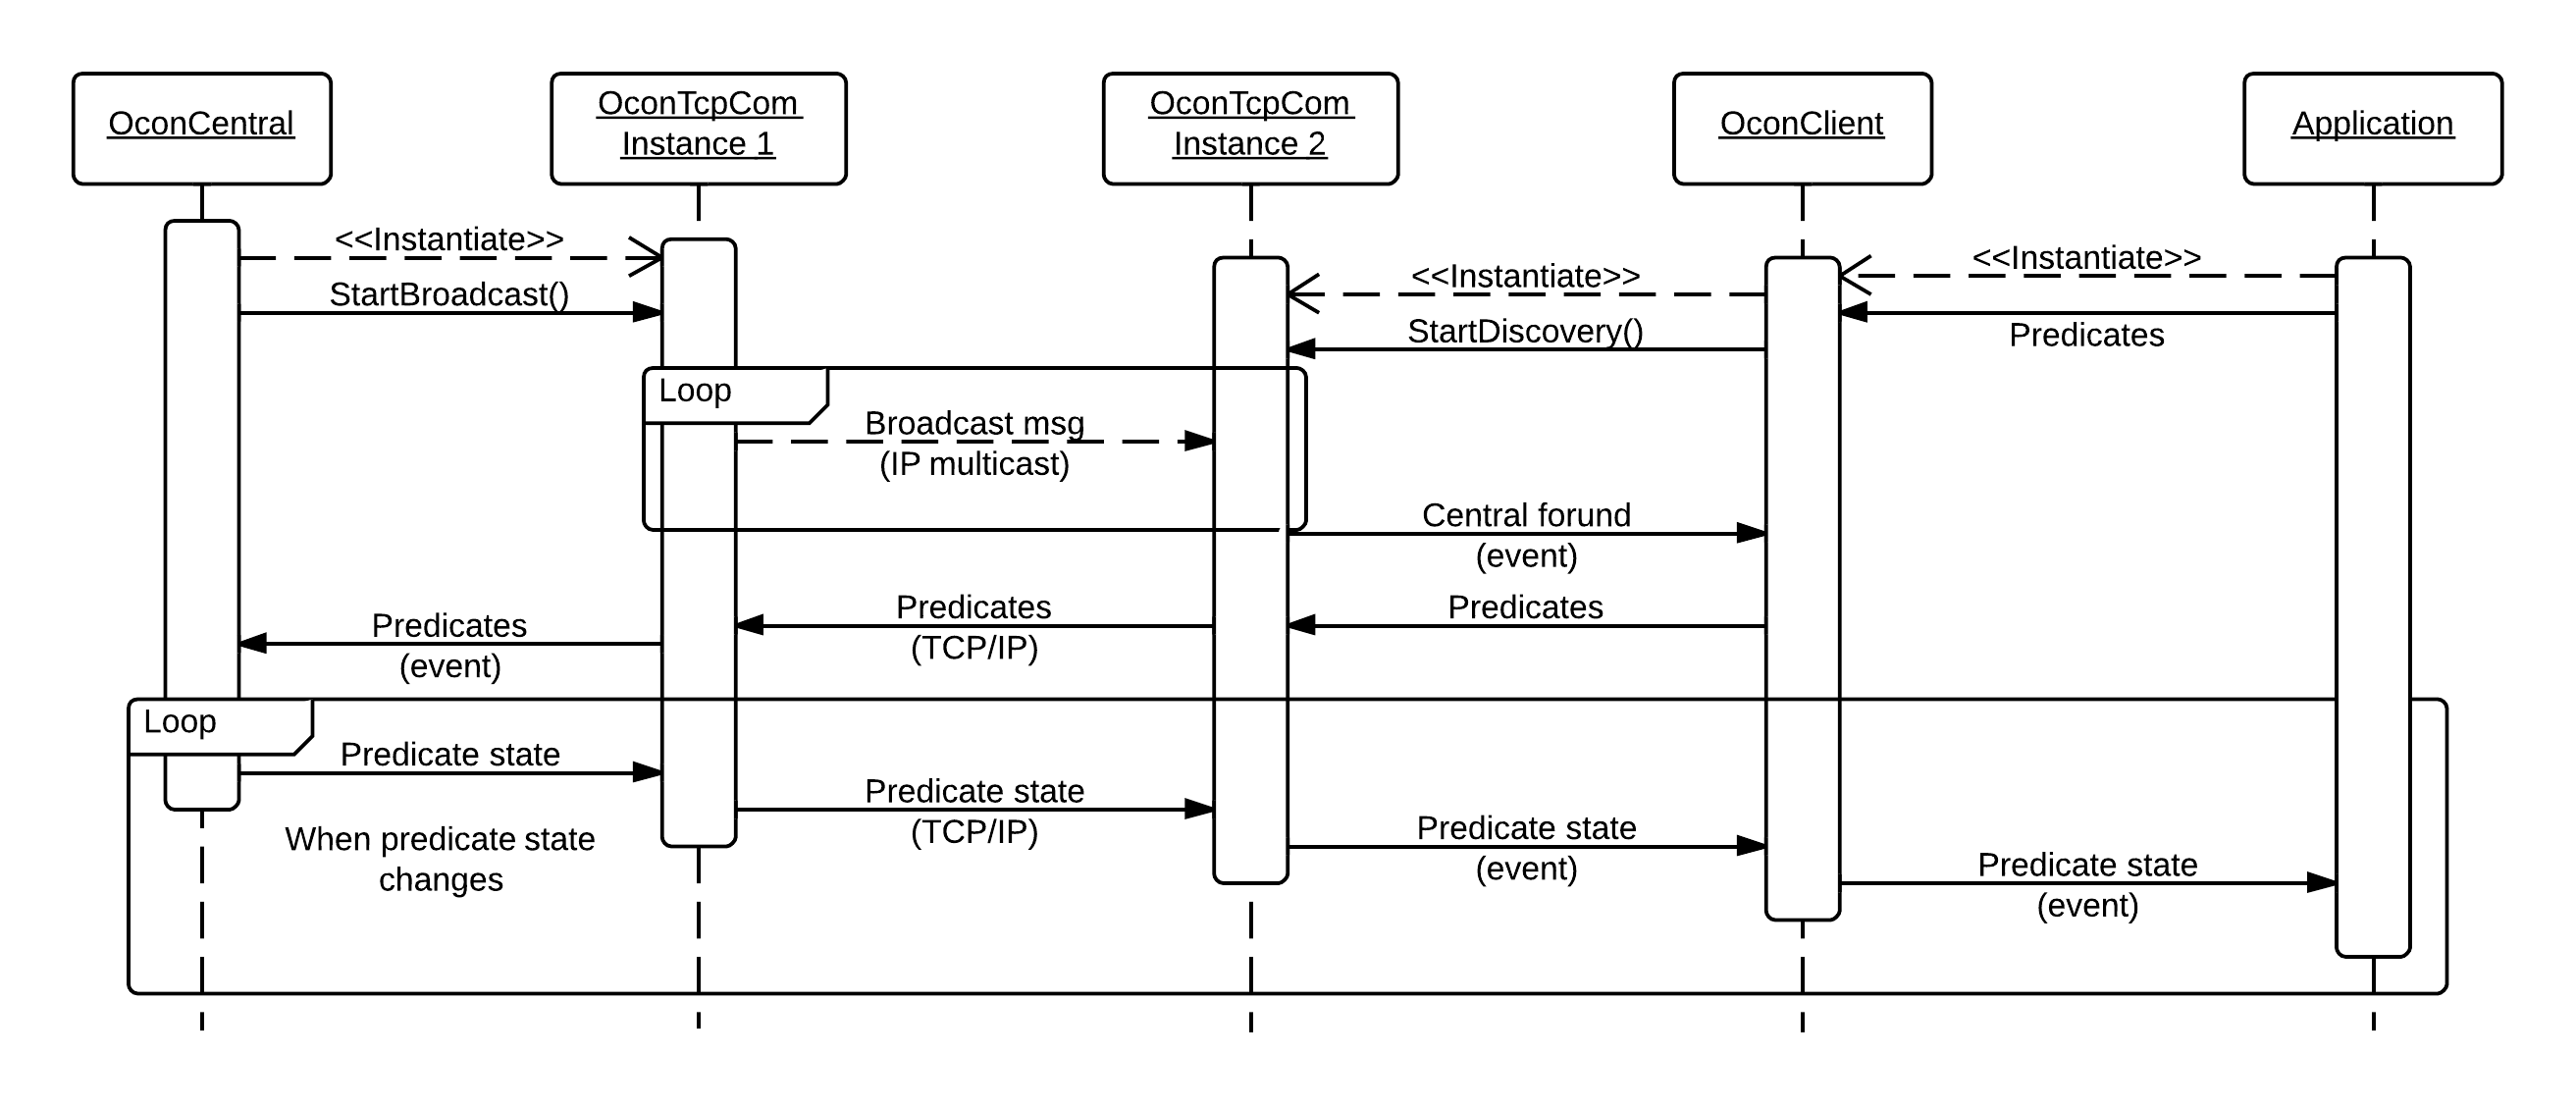
\includegraphics[width=500px]{comHelperSequence-client.png}
\caption{Client to Central sequence diagram}
\label{fig:clientComHelper}
\end{figure}

The OconClient is, as the OconWidget, very light. It contains only a constructor and a SituationStateChanged Event. The constructor takes a list of predicate identifiers as parameter, subscribes to DiscoveryServiceEvents, and starts the discovery service. When a DiscoveryServiceEvent is invoked the OconClient send its predicate identifiers to the OconCentral.

Per design the client was suppose to send a predicate and not a predicate identifier. To support clients being able to send predicates to the central, predicates must be serialized, but this is unfortunately not supported in .NET. Frameworks for handling the serialization have been researched, but none of the investigated frameworks were able serialize the predicates in Ocon as custom types are used. Therefore serializing predicates was forced out of scope. Instead of sending the predicates, they are hard coded in the central. The OconClient can then subscribe them by sending a predicate identifier. 

The OconCentral will upon receiving the predicate identifiers send back the state of the subscribed predicates. When OconClient was constructed it also subscribed IncommingSituationChanged event in the communication module. When such an event is fired OconClient will fire its SituationStateChanged event notifying subscribing applications of the predicate change.


\section{Central}
OconCentral is the core component of Ocon. The central contains a OconContextFilter and a concrete implementation of IOconCom. The context filter is aggregated of entities and situations (see figure \ref{fig:oconclassdiagram}). The implementation of a situation contains a predicate that given a set of entities can evaluate to true or false. The context filter can therefore by its set of entities evaluate the state of its situations.

\begin{figure}
\centering
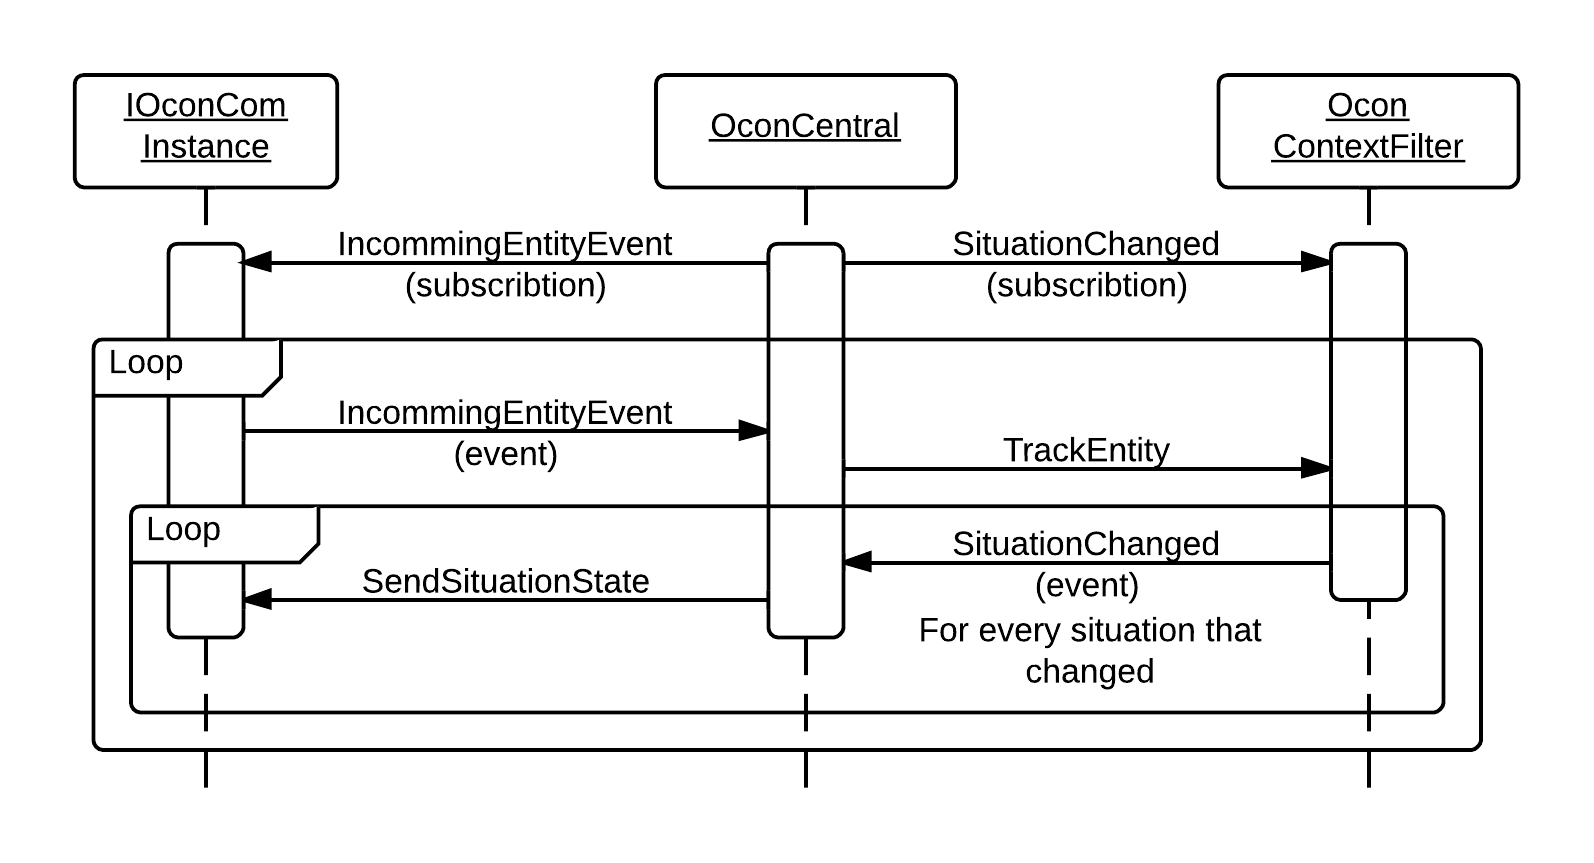
\includegraphics[width=\linewidth]{sequencediagram-central.png}
\caption{Central sequence diagram}
\label{fig:seqcentral}
\end{figure}

OconCentral is subscribing IncommingSituationSubscribtion event and when invoked the central will add the requesting peer to the given situation. It also subscribes the IncommingEntity event on IOconCom. When invoked the entity is added to the context filter and the context filter will check its predicates. If a situation changes the SituationChanged event will be fired. The central subscribing this event will when invoked call SandSituationChanged on IOconCom to notify all subscribers on the situation of its new state. This is shown in figure \ref{fig:seqcentral}

\begin{figure}
\hspace{-70px}
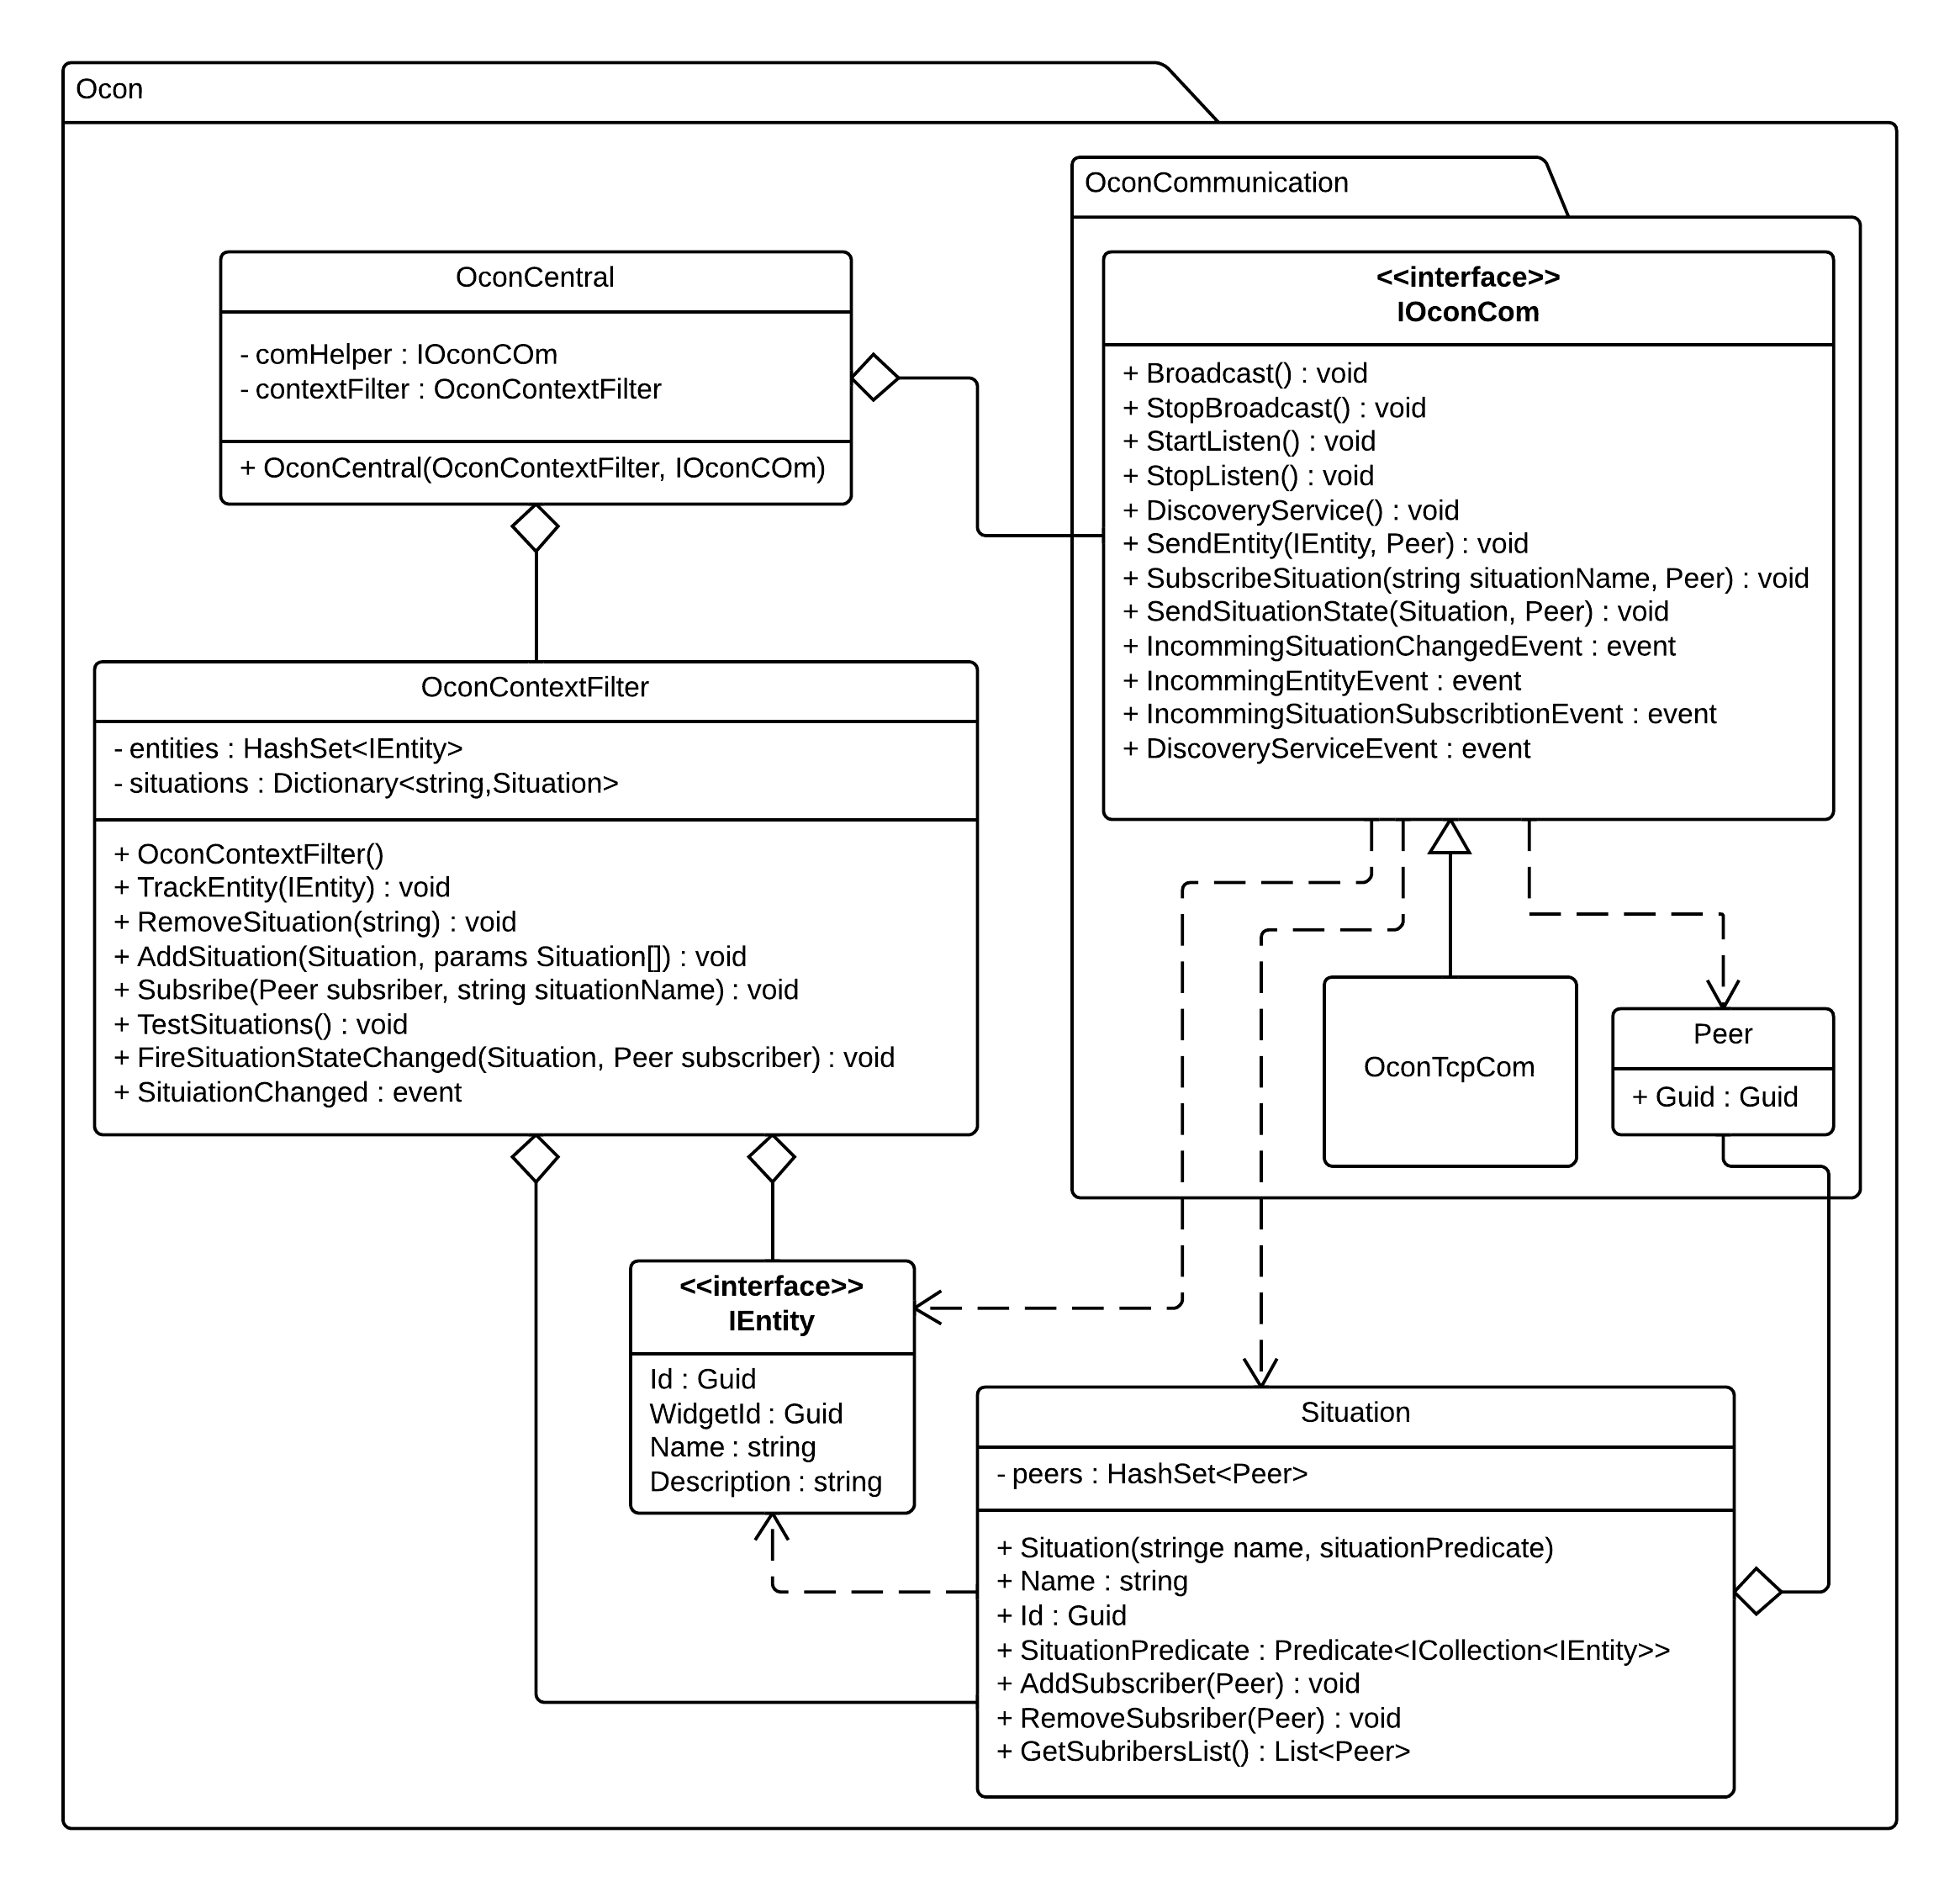
\includegraphics[width=500px]{oconclassdiagram.png}
\caption{Class diagram showing the central and its usages}
\label{fig:oconclassdiagram}
\end{figure}



\end{document}